\chapter{Hauptteil}
%

% Bis 3.1 kann weg: wurde nur zum reinkommen geschrieben

Um ein grundlegendes Verständnis für die Analyse von Dateiformaten zu entwickeln wird einem klaren Schema gefolgt. Mit diesem Schema wird sich an der chronologischen Reihenfolge von der Entstehung eines Tons bis zur Verarbeitung im Code orientiert.

\par

Jeder Ton wird durch eine Vibration erzeugt. Diese Vibration kann durch unterschiedliche Gegenstände erzeugt werden. Dazu zählen Becken eines Schlagzeugs, Saiten eines Basses oder die Stimmbänder (?).

%
\begin{enumerate}
    \item Was ist ein Ton
    \item Formen der Musikdarstellung
    \item Darstellung in der Mathematik
    \item Vorstellung Fourier Transform
    \item Ton und Fourier als Code
    \item Trennung von Instrumenten im Code
    \item Vorgehen im Projekt (evtl früher)
    \item Wie kann man auf dem Stand aufbauen? (/Wie könnte es weitergehen?)
    \item Fazit
    \begin{enumerate}
        \item Aufwand
        \item Ertrag (z.B. erworbenes Wissen)
    \end{enumerate}
\end{enumerate}
%

%
(Bis hier muss überarbeitet werden?)
%

%
\section{Formen der Musikdarstellungen}
%

%
(Einleitung und Überschriften?)
%

Musik kann unterschiedlich dargestellt werden. Je nach Bedarf, wird eine andere Form der Musikdarstellung benötigt. Eine Form der visuellen Musikdarstellung sind Musiknoten. Es ist eine formale Sprache, die vorgibt wie ein Musikstück gespielt wird \parencite{sheet_music_representations}.

\par

 - MIDI nutzt Notendarstllung

\par

Eine weitere Form der Darstellung, ist die Audiodarstellung. In diesen Darstellungen werden alle Informationen der Töne als Audiosignale digital gespeichert und geteilt. Dazu gehören auch das Timing, die Intensität, die Lautstärke, die Länge des Tons und vieles mehr. Es werden nicht die einzelnen Töne und Noten gespeichert, sondern die Frequenzen während der Aufnahme in Abhängigkeit zur Zeit. Die Audiodatei kann auch Nebengeräusche oder weitere Instrumente beihalten.

\par

Das macht es schwieriger unterschiedliche Audiosignale zu trennen und die ursprünglichen Töne wieder herzustellen. Die verbreitetste Form der Audiodarstellung ist MP3 (Quelle?). In diesem Projekt werden jedoch Wav(einheitlich?)-Dateien behandelt. Die Unterschiede, sowie Vor- und Nachteile der Audiodarstellungen werden in \cref{audio_representations} behandelt \parencite{fundamentals_of_music_processing}.

 - Musik Darstellung in Audiodateien
 - Was ist eine Note audio-/ visuell

%
\section{Was ist ein Ton?}
%

Töne entstehen durch die Vibration eines Gegenstandes. Diese erzeugen Schallwellen. Der Luftdruck einer Schallwelle wird graphisch als eine Sinus- oder Cosinusfunktion dargestellt.

%
(Spektogramm?)
%

 - Was sind Frequenzen Lautstärke etc. (Stauchung/ Streckung..., Verlauf)
 - Frequenz bei 4 Perioden/ Maxima in einer Sekunde -> 4Hz?
 - "The sinusoid can be considered the prototype of an acoustic realization of a musical note. Sometimes the sound resulting from a sinusoid is called a harmonic sound
or pure tone"

%
\section{Aufbau einer Audiodatei/ Music Representation}
%

Für die Aufnahme von Audiosignalen werden analoge Signale in eine digitale Form von Schall umgewandelt. Die analoge Signaldarstellung verwendet kontinuierliche und konstante Spannungsschwankungen, die den verursachten Luftdruckschwankungen entsprechen \parencite{digital_representation}. In der digitalen Form werden die Spannungsschwankungen als Bitstreams gespeichert und je nach Audio-Format komprimiert.

%
 - Noten sind ebenfalls musikalische Darstellung
 - Entstehung der Audiosignale: Analog/ Digital
 %

%
\subsection{Durchführung der Komprimierung}
%

Die Komprimierung von Audiodateien wird meistens verwendet, um mehr Musik auf einem Datenträger speichern zu können \parencite{what_is_audio_compression}. Um eine Aufnahme zu komprimieren wird diese in eine Sampling Rate und eine Quantisierungsgröße reduziert.

\par

%
\textbf{Sampling Rate}
%

Die Sampling Rate (/Sampling-Rate?) definiert die Anzahl von gespeicherten Signalen pro Sekunde. Dies reduziert die benötigten gespeicherten Daten von einer durchgängigen Aufnahme auf mehrere Blöcke. Beispielsweise hat eine CD Aufnahme eine Sampling Rate von 44.100 Samples pro Sekunde (kurz: 44.1 kHz), das heißt es werden 44.100 Soundsignale pro Sekunde gespeichert, dessen Übergänge kaum wahrnehmbar sind, jedoch bereits zu einem deutlichen Reduzierung des Speicherbedarfs führen.

%
(Bild einfügen?)
%

%
\textbf{Quantisierungsschrittweite}
%

Die Quantisierungsschrittweite beschreibt die Auflösung, mit der jedes Sample komprimiert wird. Die möglichen Werte eines Samples sind kontinuierlich und könnten theoretisch unendlich viele Dezimalstellen haben. Durch die Quantisierungsschrittweite werden diese Werte jedoch auf eine festgelegte Anzahl möglicher diskreter Werte reduziert, wodurch der Unterschied zwischen den Werten bestimmt wird. Bei CDs wird beispielsweise eine 16-Bit-Codierung gewählt, die 65.536 mögliche Werte definiert.

%
(Bild einfügen?)
%

%
\subsection{Waveform Audio File Format}
%

Das Waveform Audio File Format (kurz: WAV) speichert Audioaufnahmen unkomprimiert \parencite{what_is_a_wav_file}. Der Begriff leitet sich \enquote{vom englischen Wort \enquote{wave}} für Schallwelle ab \parencite{wav}. Für die in diesem Projekt behandelte (Schnelle) Fourier-Transformation sind insbesondere die \enquote{Abtastrate fs des Messsystems} und die Quantisierungsschrittweite (siehe Kapitel...?) entscheidend  \parencite{FFT_grundlagen}. Aufgrund der unkomprimierten Speicherung (und der damit verbundenen hohen Abtastrate und Quantisierungsschrittweite) lässt sich eine klare Trennung von Tonspuren ermöglichen (Referenz?).


%
\subsection{Andere Formen von Audio-Dateien}
\label{audio_representations}
%

%
\begin{itemize}
    \item MP3
    \item WMA
    \item AAC
    \item OGG
    \item FLAC
    \item RM
\end{itemize}
%

\parencite{audioformate_im_überblick}

%
\section{Trennung einer Tonspur in verschiedene Instrumente}
%

Eine Aufnahme speichert das aufgenommene Signal in Abhängigkeit zur Zeit. Jedes eingehende Signal verfügt über Schwingungen in Form von einer Amplitude. Bei einer Aufnahme vermischen sich die verschiedenen Signale zu einer gemeinsamen Amplitude und sind daher schwierig voneinander zu unterscheiden, beispielsweise bei Hintergrundgeräuschen oder der gleichzeitigen Aufnahme mehrerer Musikinstrumente. Die Trennung von Instrumenten innerhalb einer Tonspur ist ein Thema, das in Forschung und Bildung intensiv behandelt wird (Quelle?). Die am häufigsten verwendete Methode ist die Fourier-Transformation (Quelle?), die es ermöglicht, ein Signal in seine Frequenzkomponenten zu zerlegen.(Gibt es andere Vorgehensweisen?).

\par

Neben der Fourier-Transformation werden auch andere Ansätze wie die Wavelet-Transformation, die Short-Time Fourier Transform (STFT), sowie statistische Verfahren wie die Blind Source Separation (BSS) und die Independent Component Analysis (ICA) eingesetzt. Darüber hinaus finden moderne Verfahren des maschinellen Lernens, insbesondere neuronale Netzwerke, zunehmend Anwendung in der Trennung von Audiosignalen.

%
\subsection{Fourier Transformation}
%

Die Fourier Transformation ist ein Algorithmus der die Darstellung einer Tondatei verändert. Ursprünglich liegt die Audiospur mit einer Kombination aus unterschiedlichen Frequenzen in Abhängigkeit zur Zeit vor. In dieser Darstellung sind die unterschiedlichen Signale schwierig zu trennen und wird von der Fourier Transformation transformiert.

\par

%
\subsubsection{Entwicklung der Fourier Transformation}
%

Die Fourier-Transformation ist eine Generalisierung (/Verallgemeinerung?) der Fourierreihen. Diese Reihen können stetige oder stückweise stetige Funktionen in eine Summe von Sinus- und Kosinusfunktionen zerlegen. Bereits im 18. Jahrhundert wurden Fourierreihen für spezifische Funktionen entdeckt. 1822 stellte Joseph Fourier die Hypothese auf, dass sich jede Funktion als Summe solcher Reihen darstellen lässt. Erst im 20. Jahrhundert wurden Fourierreihen auch für andere stetige oder stückweise stetige Funktionen formal bewiesen. Dank der Vollständigkeiten der Funktionenreihe lässt sich die Fourier-Transformation auf eine Vielzahl von Funktionen anwenden, einschließlich periodischer und nicht-periodischer Funktionen, und erhielt ihren Namen zu Ehren von Fourier.

\par

\subsubsection{Durchführung der Transformation}

Die Fourier-Transformation ist ein mathematisches Verfahren, bei dem ein Signal aus dem Zeitbereich in den Frequenzbereich transformiert wird. Die Transformation ermöglicht es, beliebige periodische und stückweise stetige Funktionen als Summe von Sinus- und Kosinuswellen unterschiedlicher Frequenzen darzustellen.

\par

 - Vergleichsschwingungen
 
\par

In der neuen Darstellung werden die Frequenzen der Funktion unabhängig von der zeitlichen Komponente wiedergegeben. Unterschiedliche Frequenzen können unterschiedlichen Signalen zugeordnet werden. Die frequentielle Darstellung gibt an welche Signale in welchen Frequenzen Teil der Funktion sind, allerdings nicht wann. Daher wird die Darstellung wieder umgeformt in die zeitliche Abhängigkeit. 

\par

Das Signal oder die Signale, die von der Tonspur getrennt werden, können in der frequentiellen Darstellung identifiziert werden. Anschließend werden diese von den übrigen Signalen getrennt und zurück in die ursprüngliche Darstellung transformiert. Damit erhält man eine neue Tondatei, die ausschließlich aus den benötigten Signalen besteht.

\par

Anschließend werden die Tonspuren je nach Frequenz extrahiert und der Vorgang wieder rückgängig gemacht. Somit liegen diese als WAV-Datei vor und können weiterverwendet werden.

%
(Bild?)
%

\subsubsection{Parameter der Transformation}

 - Probleme:
    - Rechenaufwand/ Dauer

In (...?) wurden die relevanten Parameter wie Samplingrate und Quantisierungsschrittweite behandelt, die für die Durchführbarkeit der Transformation entscheidend sind. Zudem können verschiedene Komponenten der Transformation konfiguriert bzw. parametrisiert werden.

\par

%
\textbf{Blocklänge (/engl.?)}
%

Ein wesentlicher Parameter für die Durchführung der Fourier-Transformation ist die Blocklänge (kurz: BL), welche die Anzahl der Samples festlegt, die in der Fourier-Transformation analysiert werden.

\par

Umso länger die BL, desto präziser ist das Ergebnis der Transformation. Dies erhöht jedoch auch den Rechenaufwand und die Dauer der Transformation. In einigen Anwendungsszenarien erfordert dies eine Abwägung zwischen Verarbeitungsdauer und Genauigkeit, beispielsweise in einer App zum Stimmen von Musikinstrumenten oder zum Erkennen der gespielten Töne (Quelle?).

\par

\subsubsection{Durchführung am Beispiel einer Musiknote}

In diesem Beispiel (Müller referenzieren?) wird eine Note auf einem Piano gespielt und durch die Transformation in eine frequentielle Darstellung der gespielte Ton erkannt.

\par

Die Aufnahme des Tons ist in \cref{fig:fourier}(a) zu erkennen. Für die Transformation wird ein Ausschnitt von 10ms verwendet. Das entspricht der Blocklänge und reduziert den Rechenaufwand (referenzieren?).

\par

Anschließend werden unterschiedliche Vergleichsfunktion für die jeweiligen Frequenzen mit dem Ausschnitt der Tonspur verglichen. Die Ähnlichkeiten der jeweiligen Frequenzen werden in (f) wiedergegeben.

\par

In \cref{fig:fourier}(c) ist die Übereinstimmung für die Frequenz w = 262 Hz besonders hoch. Daraus folgt in (f) bei ungefähr 262 der höchste Wert. Die Höhe des Wertes wird in der Variable dw angegeben.

% w = ω

\par

Die Frequenz 262 entspricht der Note C4. Darüberhinaus wird bei einer Frequenz von 523 (siehe \cref{fig:fourier}(e)) eine hohe Übereinstimmung erkannt. Dies entspricht ungefähr der Frequenz des zweiten Teils der Note C4 (zweiter Teil?).

%
\begin{figure}
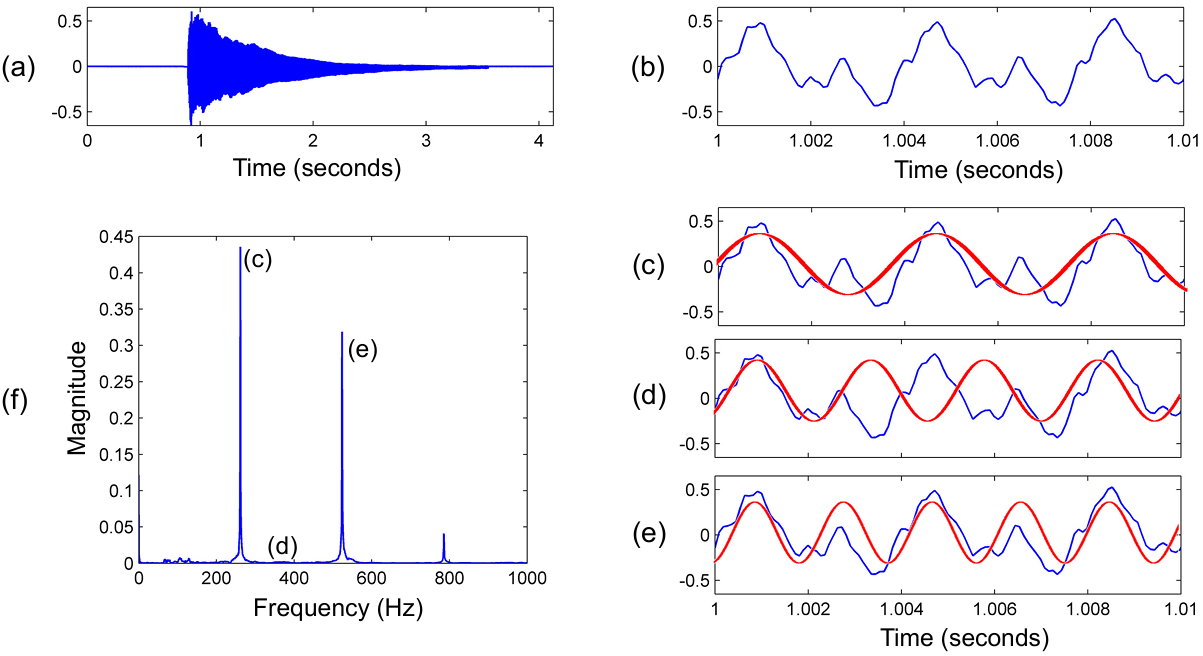
\includegraphics[width=1\textwidth]{images/Fourier_math.PNG}
\caption{Note C4 in unterschiedlichen Darstellungen}
\label{fig:fourier}
\end{figure}
% Music Processing S.41
%

%
\textbf{Nachteile}
%
    
Die Fourier Transformation ermöglicht es je nach Bedarf zwischen der zeitlichen oder der sequentiellen Darstellung zu wechseln. Allerdings ist bei der Fourier Transformation der Wechsel zwischen den Darstellung notwendig und es wird entweder die zeitliche oder die frequentielle Komponente ignoriert. Bei der Anwendung der Fourier Transformation gibt es keine Darstellung die beide Komponenten kombiniert.

    - Darstellung (nie Zeit und Frequenz)

(Noch unklar wie unterschiedliche Instrumente vorliegen, aber analoge Instrumente sollten in Sinusfunktion vorliegen und erkennbar sein)

%
\subsection{Wavelet-Transformation}
%

Die Wavelet-Transformation ist ein Vorgehen, das eine Funktion der zeitlichen Darstellung in eine 3(-?)dimensionale Darstellung in Abhhängigkeit von Zeit und Frequenz transformiert. Dafür werden Wellenfunktionen mit der ursprünglichen Funktion auf Übereinstimmungen verglichen. Es gibt unterschiedliche Wellenfunktionen und sie werden Wevelets genannt. Der Name ist aus dem französichen und wird in kleine Welle oder Wellchen übersetzt.

\par

Im Gegensatz zu der ursprünglichen Funktion sind die Flächen der Wavelets endlich und daher der Name (finite energy). Eine weitere Bedingung für Wavelets ist, dass das Integral null ergibt. Also die Fläche über und unter der X-Achse gleichgroß ist (Admissibility condition). Jedes Wavelet wird um die Parameter m und b ergänzt.

%
\begin{itemize}
    \item[m:] Bestimmt die Frequenz der Wavelet
    \item[b:] Bestimmt den Zeitpunkt der Wavelet
\end{itemize}
%

Zudem hat die Wavelet einen realen und einen imaginären Teil. Das bedeutet, dass durch die Ergänzung der imaginären Zahl die Wavelet um eine Achse ergänzt wird und 3(-?)dimensional wird. Sowohl der reale als auch der imaginäre Teil der Wavelet werden mit der Funktionen verglichen und durch die Multiplikation (Begriff?) erhält man die Ähnlichkeit der Funktion und der Wavelet.

\par

Die Ähnlichkeit der Wavelet mit der Funktion wird für jedes m und b berechnet und in dem 3-dimensionalen Ausgabe-Graphen in Abhängigkeit zur Zeit angegeben. Dies hat den Vorteil das man eine Darstellung des Signals in Abhängigkeit von Zeit und Frequenz erstellen kann.

\par

Dies kann beispielsweise sinnvoll in der Überprüfung von Ampelleuchten sein. Während die Fourier-Transformation die unterschiedlichen Frequenzen der Farben grün, gelb und rot erkennt und wiedergibt ob die drei Lichter leuchten, kann die Wavelet-Transformation angeben, ob die Lampen jeweils zum richtigen Zeitpunkt leuchten \parencite{wavelets}.

%
 - verwendet spezialisierte Funktionen: Wavelets
 - aus französisch Wellchen/ kleine Welle
 - Familie an Funktionen
   - jede für spezielle Anwendung
 - Integral unter und über X-Achse gleichgroß
   - Admissibility condition
 - endliche Fläche
   - finite energy
   - lokalisiert in Zeit